\documentclass[a4paper]{article}
\usepackage[utf8]{inputenc}
\usepackage{textcomp}
\usepackage{geometry}
\geometry{ left=2cm, right=2cm, top=2cm, bottom=2cm, bindingoffset=5mm}
\usepackage{graphicx}
\usepackage{xcolor}
\usepackage{hyperref}
\date{}
\author{}
\usepackage{fancyhdr}
\pagestyle{fancy}
\fancyhf{}
\fancyhead[R]{2973140 - Felix Bühler \\ 2892258 - Gerhard Breul \\  3141241 - Jamie Ullerich}
\fancyhead[L]{Information Visualisation and Visual Analytics \\ WS 2019/20 }
\renewcommand{\headrulewidth}{0.5pt}
\usepackage{tikz}
\usetikzlibrary{calc}
\usepackage{amsmath}
\usepackage{cleveref}
\usepackage{subcaption}

\usepackage{changepage,titlesec}
\titleformat{\section}[block]{\bfseries}{\thesection.}{1em}{}
\titleformat{\subsection}[block]{}{\thesubsection}{1em}{}
\titleformat{\subsubsection}[block]{}{\thesubsubsection}{1em}{}
\titlespacing*{\subsection} {2em}{3.25ex plus 1ex minus .2ex}{1.5ex plus .2ex}
\titlespacing*{\subsubsection} {3em}{3.25ex plus 1ex minus .2ex}{1.5ex plus .2ex}
\setcounter{MaxMatrixCols}{20}

\title{\textbf{Assignment 11}}

\begin{document}
\maketitle 
\thispagestyle{fancy}

\section*{Task 1 - Geographical Visualization}
\subsection*{a)} The main challenge with map projection is having to map a three-dimensional space (in this case, the surface of a sphere) onto a two-dimensional one without distorting crucial information. Map projections can be categorized according to which property of the sphere they represent is preserved, such as preservation of certain distances (equidistant), angles (conformal), and areas (equal-area).
\subsection*{b)} Tissot’s indicatrix is used to visualize distortions of map projections. Each area represents a circle of fixed size on the globe. 
For the Mercator projection, these areas will maintain their original round form  but become bigger towards the poles, demonstrating a preservation of angles and a distortion of area.
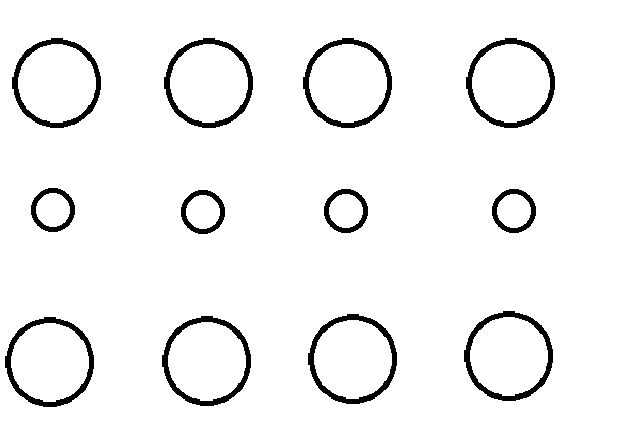
\includegraphics[width=0.7\linewidth]{Mercator} \\
Tissot’s indicatrix of the Cassini projection shows that there is no distortion for points along the central axis, however, the further a point is away from the poles, the stronger the distortion becomes, in terms of size as well as angle.
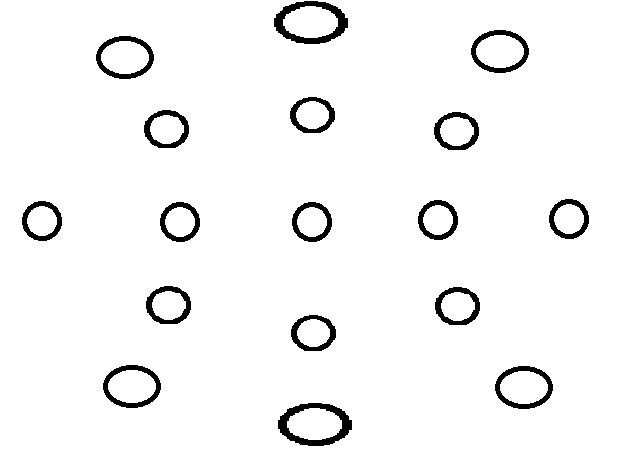
\includegraphics[width=0.7\linewidth]{Cassini}\\
\subsection*{c)} For a Dymaxion projection, the areas of Tissot’s indicatrix would maintain a similar size and shape, showing stronger distortion as they approach the edges of each projection plane. Since the angle between the plane and projection beam doesn't stray too far from 90°, distortion remains relatively low compared to e.g. a cylindrical projection at the poles. This comes at the cost of a coherent map: areas that are next to each other are often seperated by the map border.
\subsection*{d)} The important characteristic of the Mercator projection is that it is conformal, meaning it preserves angles and therefore shapes. This was relevant to nautical navigation because it meant that to follow a straight line on the map, one would simply have to sail in the same direction on the compass. While for visualization, the value of this porperty depends heavily on the given task, in many cases an accurate depiction of area would be more useful since it is often far more important to know the size of an area than its shape.
\subsection*{e)} A choropleph map conveys information about some statistical value of a geographical area, usually encoded in its coloring or shading.\\ Equal Interval Classification allows the user to determine the actual value depicted, but statistical outliers may severely impact the classification scale.\\
Quantile classification can be useful for finding the richest 10\% of a given area's population, however their actual wealth would not be visible.\\
Natural breaks classification atempts to find the most appropriate classification, generally making the classes meaningful but possibly creating arbitrary-seeming class devides in the process.
\section*{Task 2 - Kernel Density Estimation}
\begin{figure}[th!]
	\centering
	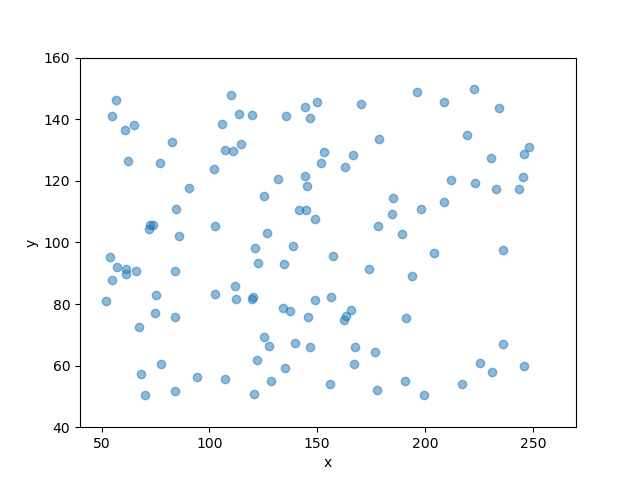
\includegraphics[width=0.7\linewidth]{scatter}
	\caption{scatter-plot}
	\label{fig:scatter}
\end{figure}

\begin{figure}[th!]
	\centering
	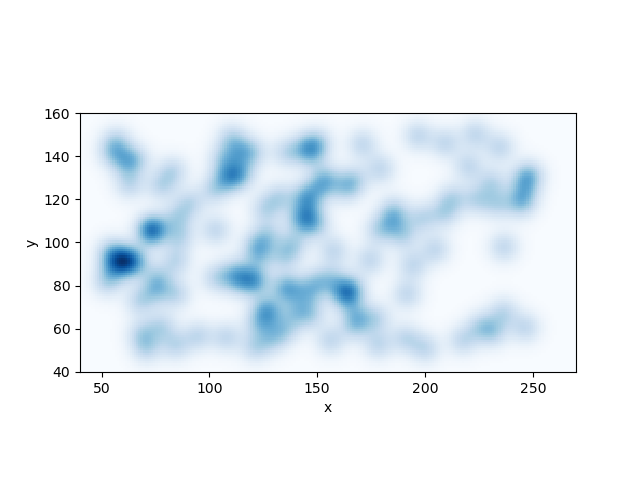
\includegraphics[width=0.7\linewidth]{density}
	\caption{kernel density estimation}
	\label{fig:density}
\end{figure}


\end{document}
